\documentclass[12pt,onecolumn,letterpaper,draftclsnofoot]{article}

\usepackage{cvpr}
\usepackage{times}
\usepackage{epsfig}
\usepackage{graphicx}
\usepackage{amsmath}
\usepackage{amssymb}
\usepackage{booktabs}
\usepackage{multirow}
\usepackage{subcaption}
\usepackage{scrextend}
\usepackage{bm}

% Include other packages here, before hyperref.

% If you comment hyperref and then uncomment it, you should delete
% egpaper.aux before re-running latex.  (Or just hit 'q' on the first latex
% run, let it finish, and you should be clear).
\usepackage[breaklinks=true,bookmarks=false]{hyperref}

\DeclareGraphicsExtensions{.pdf,.jpg,.png,.jpeg}
\graphicspath{{images/}, {figs/}}
\newcommand{\todo}[1]{\textcolor{red}{{\em [#1]}} }
\newcommand{\specialcell}[2][c]{%
    \begin{tabular}[#1]{@{}c@{}}#2\end{tabular}}
\newcommand{\secref}[1]{Section~\ref{sec:#1}}
\newcommand{\figref}[1]{Figure~\ref{fig:#1}}
\newcommand{\tabref}[1]{Table~\ref{tab:#1}}
\newcommand{\equref}[1]{Equation~\ref{equ:#1}}
\newcommand{\matr}[1]{\mathbf{#1}}
\newcommand{\bfit}[1]{\boldsymbol{#1}}
\newcommand{\bs}[1]{\boldsymbol{#1}}

\DeclareMathOperator*{\argmax}{arg\,max}
\DeclareMathOperator*{\argmin}{arg\,min}

\cvprfinalcopy % *** Uncomment this line for the final submission

\def\cvprPaperID{****} % *** Enter the CVPR Paper ID here
\def\httilde{\mbox{\tt\raisebox{-.5ex}{\symbol{126}}}}

% Pages are numbered in submission mode, and unnumbered in camera-ready
%\ifcvprfinal\pagestyle{empty}\fi
%\setcounter{page}{4321}
\begin{document}

%%%%%%%%% TITLE
\title{Sound Absorption of Rooms}

\author{Weilian Song\\
University of Kentucky\\
% {\tt\small firstauthor@i1.org}
% For a paper whose authors are all at the same institution,
% omit the following lines up until the closing ``}''.
% Additional authors and addresses can be added with ``\and'',
% just like the second author.
% To save space, use either the email address or home page, not both
}

\maketitle
%\thispagestyle{empty}

%%%%%%%%% BODY TEXT
\section{Introduction}

A lot of the music we hear today are exceptionally clear, with very little
noise that is only audible with very good listening equipment. However,
whenever we as students do a project involving audio recording, it always
sounds like there's static noise in the background. While there can be many
reasons why our recorded audio is noisy, the main issue is that the
environment in which we record at does not absorb sound very well, and can
cause unwanted noise to reflect back to the recording device or make wanted
noise diminish into nonexistance. Understanding how different rooms absorb
sound will prove useful in the future whenever audio recording is necessary,
to provide the clearest possible sound for the audience.

There are three obvious factors when determining room sound absorption level:
size, number of objects in the room, and materials of the objects and walls.
Size determines how much echo is produced when playing a sound; number of
objects in the room determines how long the sound wave has to bounce before
reaching the recording device, and materials of various objects and walls
determine the amount of sound that gets reflected or absorbed.

With the three factors as our independent variables and the sound absorption
level as our dependent variable, I hypothesize that the sound absorption level
is \textbf{higher} with:

\begin{enumerate}
  \item Smaller room (less echoic environment)
  \item More objects in the room (more bounces for the sound wave)
  \item Materials with rougher or special designed surfaces (more sound
        absorption)
\end{enumerate}

In this paper, we explore the sound absorption characteristics of three 
different rooms: a compact dormatory room, a medium classroom, and a large
classroom For each room we will be playing three sounds at different
frequencies to also determine the correlation between frequency and absorption
level.

\section{Related Work}

\paragraph{Absorption Properties of Materials} Extensive research has been
conducted to determine the sound absorption properties of various materials.
\cite{commonmaterials} Asdrubali et.\ al.\ \cite{rubber} experimented with the
absorption properties of recycled rubber crumbs from old tyres. Their
independent variables include the grain size, compaction ratio, thickness of
the end product, and bonding agent used to adhere the rubber grains together.
In their research they discovered that small sized rubber grains, purposely
developed resin, 20\% compaction ratio and thickness of 9.4 cm works the best
for sound absorption.
%
\begin{figure}
  \centering
  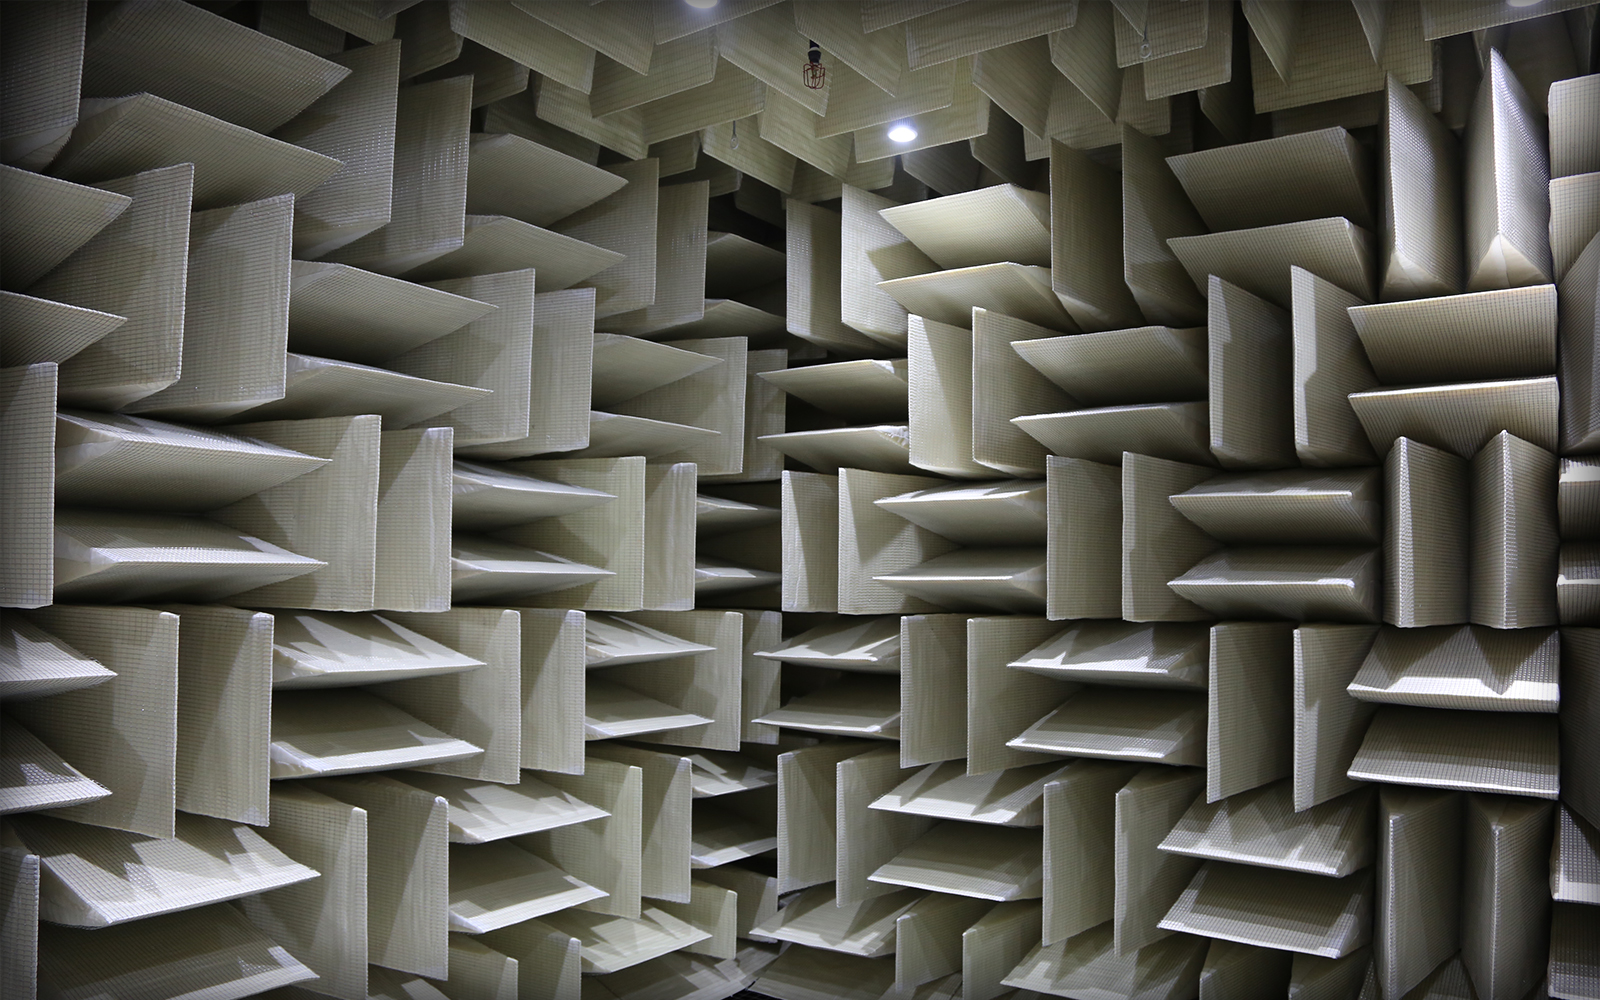
\includegraphics[width=0.5\linewidth]{chamber}
  \caption{Inside of an anechoic chamber, borrowed from \cite{anechoic}}
  \label{fig:chamber}
\end{figure}

\paragraph{Room Absorption} 
Room sound absorption can be expressed in terms of the room's sound absorption
coefficient. As explained in \cite{acousticcoeff}, given that we know the room
walls' materials, we can perform a lookup of each material's sound absorption
coefficient $\alpha$ through the provided table in \cite{acousticcoeff}, and
calculate the total room sound absorption $A$ with the following equation:
%
\begin{equation}
  A = \sum_{i} S_i \alpha_i
\end{equation}
%
where $S_i$ is the total area of material $i$ in unit $m^2$ and $\alpha_i$ is
the sound absorption coefficient for material $i$. Mean absorption coefficient
for every $m^2$ of the room can be calculated through dividing $A$ by the
total area of the room.

Sound absorption coefficient is a good way to measure a room's acoustic
niceness, as it provides a quantifiable metric for comparing rooms with
different sizes and materials.

Different materials within the room will absorb different amounts of sound.
Objects that has loose structures like various types of wool and foam has
higher absorption coefficients, while materials like glass, sheets of wood and
cork sheet has lower absorption coefficients. Interestingly, snow has a
relatively high absorption coefficient, at 0.75.

\paragraph{Anechoic Chamber}
For recording and research purposes, there are rooms specifically designed for
maximum sound absorption, which are called anechoic chambers, as shown in
\figref{chamber}. Construction of a world-class anechoic chamber is extremely
tedious, having to consider many aspects like location of the chamber, size of
the room, materials of the wall, custom parts, etc. The eStudio on campus also
has a small anechoic chamber, elevated off the ground for less transmitted
vibration and lined with foam sound absorption materials on the inside to
remove echo.

\paragraph{Recording Methods}
As the experiment requries recording of audio, some knowledge of how to setup
the recording equipment is necessary. \cite{recording} shows a setup that uses
three microphones and an impedance tube to measure the acoustic and
non-acoustic properties of various materials. While the experiment presented
in this paper does not require an elaborate setup, it still helps with
understanding best practices.

\section{Methods}
The goal of the experiment is to identify the effect of room sizes, object
density and materials on sound absorption. To achieve that goal, three rooms
with different properties are chosen: small, medium and large. The small room
is my dorm room, which is compact, non-echoic and has smooth walls with dense
object arrangements. The medium room is a medium classroom, which is slightly
echoic and is relatively open. Finally the large room is a large classroom,
with rough brick walls, echoic room characteristics and sparse object
arrangements.

To measure the sound absorption level of the room, a microphone and a speaker
is placed in the center of the room, with the speaker and the microphone
placed a set distance apart. The distance is maintained for all three rooms. A
simple overview of the setup is shown in \figref{setup}.
%
\begin{figure}
  \centering
  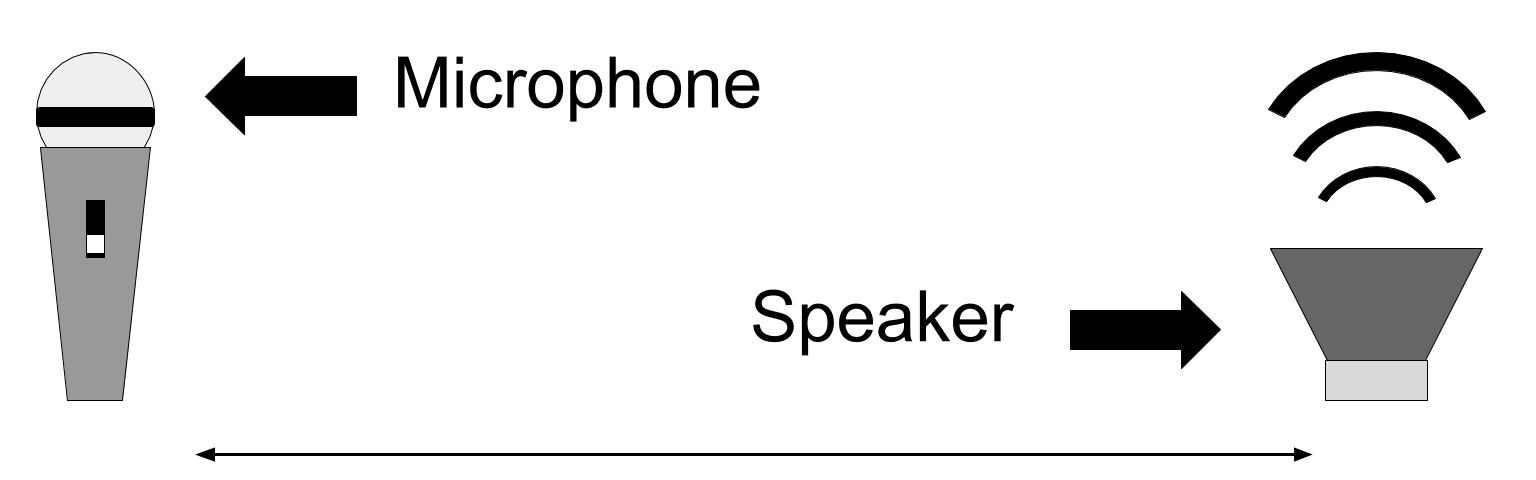
\includegraphics[width=0.5\linewidth]{setup}
  \caption{Experiment setup}
  \label{fig:setup}
\end{figure}
%
Four measurements are taken for each room, one with the speaker turned off
(ambient noise), and three with the speaker playing sound at 500, 2000 and
4000 Hz. The purpose of the different sound frequencies is to discover if they
are different in terms of percentage of absorption. Each measurement is ten 
seconds long, and with three different rooms, a total of twelve audio clips
are recorded.

\section{Experiment}

\subsection{Equipment and Data Collection}
For the recording device, a Blue Yeti microphone is used, with gain set at
100\% and pickup pattern set in omnidirectional mode. The reason for
omnidirectional pickup is to allow the microphone to record audio 360 degree
wise, including audio that bounces off the walls before hitting the
microphone. For the speaker, an iPhone is used, playing the three frequencies
at max volume. The iPhone speaker is pointed straigt up, so sound waves may
fill the entire room. To record the audio, the microphone is plugged into a
laptop and a simple python script is used to save the recorded audio clips.

Audio data is sampled at 44199 Hz/sec, and with 10 seconds of
audio data, each clip results in 441990 data points. The first and last
quarter of the data is discarded, as it is often noisy due to me clicking the
record button on the laptop. To analyze the recorded audio clips, another
python script is used to first normalize the data points to be between $-1$
and $1$, and then calculate the average of all the non-negative values. The
reason I removed the negative ones is because due to the periodic properties
of sound wave, the audio data is fairly symmetric across the x-axis, and
averaging all values would result in a near-zero value. The same analysis
process is done for each audio clip, for each room.

\subsection{Results and Discussion}
\tabref{results} displays the results for each of the three rooms. The ambient
column is mostly for assurance that the ambient noise at each of the three
locations are not drastically different from each other. The large room seems
to absorb the least when playing sound at 500 and 4000 kHz, as evident of the
largest average normalized frequency values. The small room seems to absorb
the least when playing sound at 2000 kHz. This is an interesting phenomenon,
as I expected the large room to absorb the most for all three frequencies,
with the room being very echoic and sound energies bouncing back to the
micrphone. In contrast, the small room should absorb the least, as the space
is more confined and sound waves can travel back to the microphone with
greater potential.

As the results are drastically different from my hypothesis, it is difficult
to determine the cause for such phenomenon. For the large room to have such
poor sound absorption at 500 and 4000 kHz, I suspect that since the room is
very echoic and is relatively sparse with objects, the sound waves can travel
back and forth without any issue. For the small room to have such poor sound
absorption at 2000 kHz, I suspect that the frequency played a major role. It
would take more experimentation to determine how frequency affects sound
absorption, but that is beyond the scope of this paper.

\section{Conclusion}
Sound absorption is an important subject in many ways, including construction
of professional sound booths, research in acoustic fields, etc. In this paper,
three independent variables are chosen to conduct acoustic experiments in, and
as a result three rooms are picked to assess their sound absorption level.
From analysis, a medium sized room with relatively sparse object layout has
the most consistent sound absorption level across all frequencies, which is
ideal for audio recording. Further research needs to be conducted to verify
results, and more independent variables need to be assessed to determine their
affect.

\begin{table}[]
\centering
\caption{Results for each room playing different frequencies, higher value
  means less sound absorption}
\label{tab:results}
\begin{tabular}{ccccc}
	\toprule
	Room   & Ambient & 500            & 2000           & 4000           \\
  \hline
	Small  & 0.010   & 0.021          & \textbf{0.167} & 0.098          \\
	Medium & 0.013   & 0.012          & 0.087          & 0.052          \\
	Large  & 0.004   & \textbf{0.064} & 0.133          & \textbf{0.181}
	\bottomrule
\end{tabular}
\end{table}

{\small
\bibliographystyle{ieee}
\bibliography{biblio}
}

\end{document}
